\section*{Mating e saggio di complementazione}

	\subsection*{Introduzione}
	L'esperienza prevede l'utilizzo di tre diversi ceppi di \emph{Saccharomyces cerevisiase} in forma aploide e di studiare l'avvenuta complementazione.
	I ceppi presentavano auxotrofie specifiche e differenziate tra di loro, in modo da riuscire a creare terreni selettivi che permettessero di escludere tutte le cellule che non avessero effettuato complementazione.
	
		\subsubsection*{Ceppi utilizzati}
		\begin{center}
			BY4704 \emph{Mata, ade$2\Delta$::hisG his$3\Delta200$ leu$2\delta 0$ lys$2\Delta0$ met$15\Delta0$ trp$1\Delta63$}
		\end{center}
		\begin{center}
			yIG397 \emph{MAT$\alpha$, ade2-1 leu2-3,112 trp1-1 his3-11,15 can1-100 URA3::exRGC::p-cyc1::ADE2:: ura3-1}
		\end{center}
		\begin{center}
			E134 \emph{MAT$\alpha$, ade5-1 his7-2 leu2-3,112 trp1-289 ura3-52 lys2::insE-A14}
		\end{center}

		\subsubsection*{Ottenere cellule diploidi}
		Le piastre contenenti le cellule pronte per compiere la complementazione si ottengono attraverso \emph{Replica plating}.
		Vengono poste sul velluto due piastre contenenti due patches.
		La prima piastra conteneva una patch con il ceppo BY4704 e un'altra con yIG397.
		La seconda piastra conteneva invece una patch con il ceppo E134 e un'altra con yIG397.
		Le piastre vengono disposte in modo che le patches di ogni piastra siano perpendicolari tra di loro a formare un ``hashtag'' ($\#$).
		Le zone di incontro tra le patch diverse sono le zone dove avviene complementazione.
		Si ottengono pertanto zone di complementazione per:
		\begin{multicols}{4}
			\begin{itemize}
				\item BY4704-E134.
				\item E134-yIG397.
				\item yIG397-yIG397.
				\item yIG397-BY4704.
			\end{itemize}
		\end{multicols}

		\subsubsection*{Selezione delle cellule diploidi}
		Dopo aver effettuato le impronte sul velluto queste vengono replicate su piastre contenenti terreni diversi: uno completo di controllo (YPDA) e uno selettivo. 
		Il terreno selettivo viene scelto in base al genotipo per sfruttare il fenomeno di complementazione.

		\subsubsection{Analisi del genotipo}
		Lo scopo dell'analisi del genotipo \`e evidenziare auxotrofie che verrebbero mascherate dalla complementazione.
		\begin{center}
			\begin{tabular}{|c|c|c|c|c|c|c|c|c|c|}
				\hline
				Ceppo & Mat & \multicolumn{8}{c|}{Genotipo}\\
				\hline
				BY4704 & \emph{a} & \emph{ade2} & \emph{his3} & \emph{leu2} & \emph{lis2} & \emph{met15} & \emph{trp1} & & \\
				\hline
				E134 & $\alpha$ & \emph{ade5-1} & \emph{his7-2} & \emph{leu2-3} & \emph{lis-2} & & \emph{trp1-289} & \emph{ura3-52} & \\
				\hline
			\end{tabular}
		\end{center}
		\begin{center}
			\begin{tabular}{|c|c|c|c|c|c|c|c|c|c|}
				\hline
				Ceppo & Mat & \multicolumn{8}{c|}{Genotipo}\\
				\hline
				BY4704 & \emph{a} & \emph{ade2} & \emph{his3} & \emph{leu2} & \emph{lis2} & \emph{met15} & \emph{trp1} & & \\
				\hline
				yig397 & $\alpha$ & \emph{ade2-1} & \emph{his3-11} & \emph{leu2-3} & & & \emph{trp1-1} & & \emph{can1-100}\\
				\hline
			\end{tabular}
		\end{center}
		\begin{center}
			\begin{tabular}{|c|c|c|c|c|c|c|c|c|c|}
				\hline
				Ceppo & Mat & \multicolumn{8}{c|}{Genotipo}\\
				\hline
				E134 & $\alpha$ & \emph{ade5-1} & \emph{his7-2} & \emph{leu2-3} & \emph{lis-2} & & \emph{trp1-289} & \emph{ura3-52} & \\
				\hline
				yig397 & $\alpha$ & \emph{ade2-1} & \emph{his3-11} & \emph{leu2-3} & & & \emph{trp1-1} & & \emph{can1-100}\\
				\hline
			\end{tabular}
		\end{center}


		\subsubsection*{Risultati aspettati}

			\paragraph*{Complementazioni possibili}
			Si nota come nelle patch yIG397-yIG397 e E134-yIG397 non avviene complementazione in quanto presentano lo stesso tipo sessuale.
			Le complementazioni che possono avvenire sono pertanto tra:
			\begin{multicols}{2}
				\begin{itemize}
					\item BY4704-E134
					\item yIG397-E134
				\end{itemize}
			\end{multicols}

			\paragraph*{Scelta del terreno selettivo per la selezione del diploide}
			Analizzando le auxotrofie delle forme aploidi mascherate durante la complementazione si pu\`o determinare un terreno che permetta unicamente la sopravvivenza dell'organismo diploide che ha subito complementazione.
				
				\subparagraph*{BY4704-E134}
				Le auxotrofie mascherate nell'organismo diploide sono quelle per:
				\begin{multicols}{4}
					\begin{itemize}
						\item Adenosina.
						\item Istidina.
						\item Metionina
						\item uracile.
					\end{itemize}
				\end{multicols}
				L'organismo diploide, oltre ad essere sensibile alla canamicina rimane auxotrofo per:
				\begin{multicols}{3}
					\begin{itemize}
						\item Leucina.
						\item Lisina.
						\item Triptofano.
					\end{itemize}
				\end{multicols}
				Un possibile terreno selettivo per il diploide BY4704-E134 sarebbe privo di:
				\begin{multicols}{4}
					\begin{itemize}
						\item Adenosina.
						\item Istidina.
						\item Metionina
						\item Uracile.
						\item Canamicina.
					\end{itemize}
				\end{multicols}
				Mentre conterrebbe:
				\begin{multicols}{3}
					\begin{itemize}
						\item Leucina.
						\item Lisina.
						\item Triptofano.
					\end{itemize}
				\end{multicols}

				\subparagraph*{BY4704-yIG397}
				Le auxotrofie mascherate nell'organismo diploide sono quelle per:
				\begin{multicols}{2}
					\begin{itemize}
						\item Metionina
						\item Lisina.
					\end{itemize}
				\end{multicols}
				L'organismo diploide perde inoltre la sensibilit\`a alla canamicina.
				Rimarrebbe inoltre auxotrofo per:
				\begin{multicols}{4}
					\begin{itemize}
						\item Adenina.
						\item Istidina.
						\item Leucina.
						\item Triptofano.
						\item Uracile.
					\end{itemize}
				\end{multicols}
				Si nota inoltre come non \`e possibile, con queste conoscenze genotipiche determinare un terreno capace di selezionare il diploide eliminando entrambi gli organismi aploidi da cui si \`e generato.
	\subsection*{Risultati}
	
		\begin{figure}[H]
			\centering
			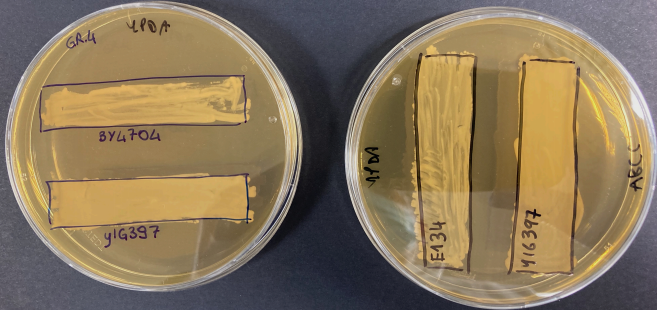
\includegraphics[scale=0.4]{./Pics/SelezioneDiploidi/Giorno1-patch-terreno-ricco.png}
			\caption{Patch di colture diploidi su terreno singolo}
			\label{fig1}
		\end{figure}
	\begin{multicols}{2}
		\begin{figure}[H]
			\centering
		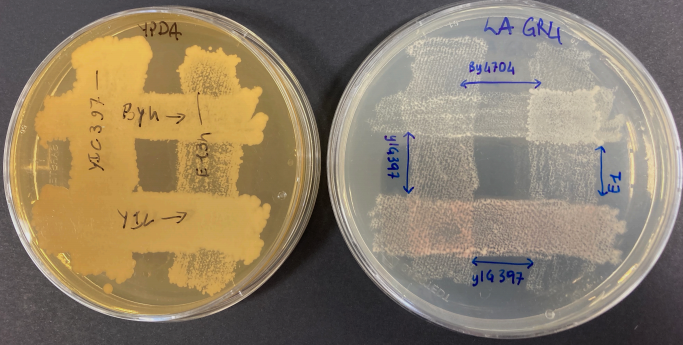
\includegraphics[scale=0.3]{./Pics/SelezioneDiploidi/Giorno2-selezione.png}
		\caption{Colture di replica consecutiva su piastra non selettiva YPDA (destra) e selettiva hA (sinistra)}
		\label{fig2}
	\end{figure}
	\columnbreak
		\begin{figure}[H]
			\centering
		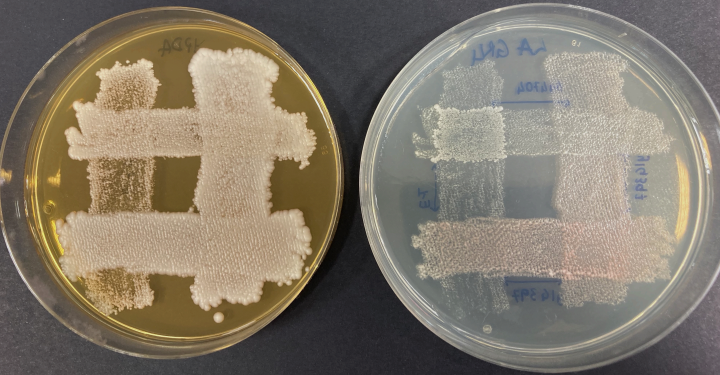
\includegraphics[scale=0.275]{./Pics/SelezioneDiploidi/Giorno2-selezione-face-up.png}
		\caption{Colture face up di replica consecutiva su piastra non selettiva YPDA (destra) e selettiva hA (sinistra)}
		\label{fig3}
	\end{figure}
	\end{multicols}

	\subsection*{Considerazioni finali}
	Si notano i risultati dell'esperimento nelle figure ~\ref{fig2} ~\ref{fig3}.
	Queste mostrano infatti l'incubazione delle colture ottenute dopo replica plating.
	Si nota come la crescita della coltura non \`e stata influenzata nel terreno completo, con alta densit\`a per tutti i ceppi e le complementazioni.
	Nel terreno selettivo hA, in assenza di istidina si nota una scarsa presenza dei ceppi BY4704 e E134, auxotrofi per istidina, mentre si nota crescita dove le loro patch si incontrano.
	Questa coltura dimostra l'avvenuta complementazione dei due ceppi e la buona riuscita dell'esperimento.
	
		\subsubsection*{Metodi alternativi per selezionare BY4704-yIG397}
		L'impossibilit\`a di selezionare attraverso il genotipo pone la necessit\`a di trovare un altro metodo per isolarlo.
		Una proposta nata durante il lavoro \`e stata quella di mettere in eccesso il ceppo BY4704 in modo da massimizzare la probabilit\`a che tutto il ceppo yIG397 venga complementato.
		Successivamente si pu\`o eliminare BY4704 sfruttando la sua sensibilit\`a alla canamicina.
		Questo metodo presenta per\`o una criticit\`a importante: non assicura in alcun modo che tutto il yIG397 sia complementato, tenta unicamente di renderlo molto probabile.
	
